\documentclass[10pt,A4paper,tikz,border=10pt]{standalone}
\usepackage[utf8]{inputenc}
\usepackage[T1]{fontenc}
\usepackage{amsmath}
%\usepackage{amsfonts}
\usepackage{amssymb}
\usepackage{mathtools}
\DeclarePairedDelimiter\abs{\lvert}{\rvert}
\usepackage{tikz}
\usetikzlibrary{shapes,arrows,shapes.misc,shapes.symbols}
\usetikzlibrary{positioning}
\usepackage{gitinfo2}
\usepackage{graphicx}

\makeatletter
\AddToShipoutPictureBG{%
	\AtPageLowerLeft{%
		\kern2.6cm
		\raisebox{\dimexpr.5\paperheight-.8\height}
		{\rotatebox{90}{\gitMarkFormat\gitMarkPref{} \textbullet{} \gitMark}}%
	}%
}%
\makeatother
\newcommand{\prdfrazioni}{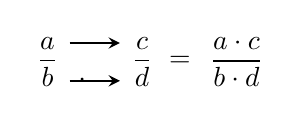
\begin{tikzpicture}[thick]
		\def\x{2.8mm}
		\def\h{2.4mm}
		\def\dist{12mm}%1cm
		\node at (0,0) {$\displaystyle \frac{a}{b}$};
		\node at (\dist,0) {$\displaystyle \frac{c}{d}$};
		\node at (1.4*\dist,0) {$\displaystyle =$};
		\node at (2.0*\dist,0) {$\displaystyle \frac{a\cdot c}{b\cdot d}$};
		% collegamento termini
		\draw[-stealth] (\x, \h)--(\dist-\x,\h); 
		\draw[-stealth] (\x,-\h)--node [near start] {$\cdot$}(\dist-\x, -\h);
	\end{tikzpicture}%
}
%\renewcommand{\gitMarkFormat}{\color{blue}\sffamily\bfseries}
\begin{document}
\tikzset{
	decision/.style={diamond, draw, %fill=blue!20,
		text width=5.5em, text badly centered, 
		%node distance=2.5cm
		, inner sep=0pt
	},
	block/.style={rectangle, draw, %fill=blue!20,
		text width=10em, 
		text centered, 
		%node distance=2.0cm,
		%rounded corners, 
		%minimum height=3em
	},
	loop/.style={chamfered rectangle,chamfered rectangle 	xsep=2cm, draw, %fill=blue!20,
		text width=15em, text centered,  
		node distance=2.5cm,% minimum height=3em
	},
	cloud/.style={draw, ellipse,%fill=red!20, 
		%node distance=1.5cm,
		 minimum height=2em
	},
	input/.style={ % requires library shapes.geometric
		draw,
		%node distance=1.5cm,
			text width=10em, text centered,  
		trapezium,
		trapezium left angle=60,
		trapezium right angle=120,
	},
	line/.style={draw, very thick, %color=black!50,
		-latex'},
	print/.style={ % requires library shapes.symbols
		draw,
		text width=14em, 
		text centered,  
		tape,
		tape bend top=none
	},
connessione/.style={
draw,
circle,
radius=5pt,
}
}
%	\begin{center}

		\begin{tikzpicture}[scale=1, %node distance = 2.5cm,
			 auto]
			% Place nodes
			\node [cloud] (init) {Inizio};
			\node [input, below of=init, node distance=2cm] (passo1) {Leggo la 
			disequazione $ax^2+bx+c\quad \text{Verso}\quad 0$};
		\node [block, below of=passo1, node distance=2cm] (passo2) {Risolvo 
		l'equazione $ax^2+bx+c=0$};
	\node [decision, below of=passo2, node distance=2cm] (passo3) 
	{$\Delta>0$};
	\node [decision, right of=passo3, node distance=3.5cm] (passo3Si) 
	{$a>0$};
	\node [block, right of=passo3Si, node distance=3.8cm] (passo3SiSi) 
	{\begin{tikzpicture}[line cap=round,line join=round,>=triangle 
	45,x=1.0cm,y=1.0cm]
			\draw[->,color=black] (-2,0) -- (1.5,0);
			\clip(-2,-0.3) rectangle (1.5,0.5);
			\draw (-1.0,0.5)-- (-1.0,0);%bandiera x1
			\draw (0.5,0.5)-- (0.5,0);%bandiera x2
\draw [line width=1.2pt,dash pattern=on 5pt off 5pt] (-1.0,0.5) --(0.5,0.5);
			\draw (0.5,0.5)-- (2,0.5); %dopo x2
			\draw (-2,0.5)-- (-1.0,0.5); %prima x1
			\draw (-1.2,0.02) node[anchor=north west] {$x_1$};
			\draw (0.3,0.02) node[anchor=north west] {$x_2$};
	\end{tikzpicture}};
\node [block, below of=passo3Si, node distance=2.5cm] (passo3SiNo) 
{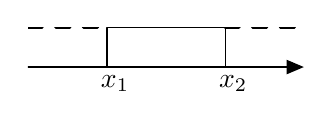
\begin{tikzpicture}[line cap=round,line join=round,>=triangle 
		45,x=1.0cm,y=1.0cm]
		\draw[->,color=black] (-2,0) -- (1.5,0);
		\clip(-2,-0.3) rectangle (1.5,0.5);
		\draw (-1.0,0.5)-- (-1.0,0);%bandiera x1
		\draw (0.5,0.5)-- (0.5,0);%bandiera x2
		\draw (-1.0,0.5) --(0.5,0.5);
		\draw [line width=1.2pt,dash pattern=on 5pt off 5pt]  (0.5,0.5)-- 
		(2,0.5); %dopo x2
		\draw [line width=1.2pt,dash pattern=on 5pt off 5pt] (-2,0.5)-- 
		(-1.0,0.5); %prima x1
		\draw (-1.2,0.02) node[anchor=north west] {$x_1$};
		\draw (0.3,0.02) node[anchor=north west] {$x_2$};
\end{tikzpicture}};
\node [decision, below of=passo3, node distance=5cm] (passo4) 
{$\Delta=0$};
\node [decision, right of=passo4, node distance=3.5cm] (passo4Si) 
{$a>0$};
	\node [block, right of=passo4Si, node distance=3.8cm] (passo4SiSi) 
{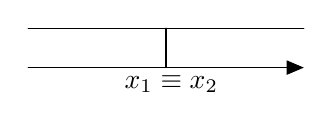
\begin{tikzpicture}[line cap=round,line join=round,>=triangle 
		45,x=1.0cm,y=1.0cm]
		\draw[->,color=black] (-2,0) -- (1.5,0);
	%	\clip(-2,-0.3) rectangle (1.5,0.5);
		\draw (-0.25,0.5)-- (-0.25,0);%bandiera x1
		\draw (-2,0.5)-- (1.5,0.5); %prima x1
		\draw (-.9,0.02) node[anchor=north west] {$x_1\equiv x_2$};
\end{tikzpicture}};
	\node [block, below of=passo4Si, node distance=2.5cm] (passo4SiNo) 
{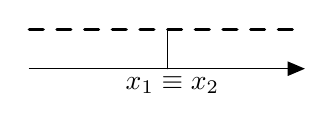
\begin{tikzpicture}[line cap=round,line join=round,>
		=triangle 
		45,x=1.0cm,y=1.0cm]
		\draw[->,color=black] (-2,0) -- (1.5,0);
	%	\clip(-2,-0.3) rectangle (1.5,0.5);
		\draw (-0.25,0.5)-- (-0.25,0);%bandiera x1
		\draw [line width=1.2pt,dash pattern=on 5pt off 5pt] (-2,0.5)-- 
		(1.5,0.5); %prima x1
		\draw (-.9,0.02) node[anchor=north west] {$x_1\equiv x_2$};
\end{tikzpicture}};
\node [decision, below of=passo4, node distance=5cm] (passo5) 
{$\Delta<0$};
\node [decision, right of=passo5, node distance=3.5cm] (passo5Si) 
{$a>0$};
	\node [block, right of=passo5Si, node distance=3.8cm] (passo5SiSi) 
{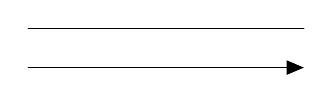
\begin{tikzpicture}[line cap=round,line join=round,>=triangle 
		45,x=1.0cm,y=1.0cm]
		\draw[->,color=black] (-2,0) -- (1.5,0);
	%	\clip(-2,-0.3) rectangle (1.5,0.5);
	%	\draw (-0.25,0.5)-- (-0.25,0);%bandiera x1
		\draw (-2,0.5)-- (1.5,0.5); %prima x1
	%	\draw (-.9,0.02) node[anchor=north west] {$x_1\equiv x_2$};
\end{tikzpicture}};
	\node [block, below of=passo5Si, node distance=2.5cm] (passo5SiNo) 
{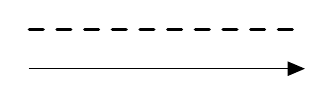
\begin{tikzpicture}[line cap=round,line join=round,>
		=triangle 
		45,x=1.0cm,y=1.0cm]
		\draw[->,color=black] (-2,0) -- (1.5,0);
	%	\clip(-2,-0.3) rectangle (1.5,0.5);
	%	\draw (-0.25,0.5)-- (-0.25,0);%bandiera x1
		\draw [line width=1.2pt,dash pattern=on 5pt off 5pt] (-2,0.5)-- 
		(1.5,0.5); %prima x1
%		\draw (-.9,0.02) node[anchor=north west] {$x_1\equiv x_2$};
\end{tikzpicture}};
	\node [connessione, below of=passo5, node distance=3.5cm] (Connessione){};
	\node [block, below of=Connessione,node distance=1.5cm] (Passo6) {Leggo la 
	domanda e 
	utilizzando il grafico rispondo}; 
	\node [cloud, below of=Passo6,node distance=1.5cm] (stop) {Fine}; 
%	\node [cloud, below of=nodo5] (stop) {Fine};5
			\path [line] (init) -- (passo1);
			\path [line] (passo1) -- (passo2);
     		\path [line] (passo2) --  (passo3);
     		\path [line] (passo3) -- node[near start] {Si} (passo3Si);
     		\path [line] (passo3Si) -- node[near start] {Si} (passo3SiSi);
     		\path [line] (passo3) -- node[near start] {No} (passo4);
     		\path [line] (passo3Si) -- node[near start] {No} (passo3SiNo);
     		\path [line] (passo4) -- node[near start] {Si} (passo4Si);
     		\path [line] (passo4Si) -- node[near start] {Si} (passo4SiSi);
     		\path [line] (passo4) -- node[near start] {No} (passo5);
     		\path [line] (passo4Si) -- node[near start] {No} (passo4SiNo);
     		\path [line] (passo5) -- node[near start] {Si} (passo5Si);
     		\path [line] (passo5Si) -- node[near start] {Si} (passo5SiSi);
     		\path [line] (passo5) --  (Connessione);
     		\path [line] (passo5Si) -- node[near start] {No} (passo5SiNo);
     		\path [line] (Connessione) --  (Passo6);
     		\path [line] (Passo6) --  (stop);
			\path[line] (passo3SiSi.east)--node[near 
start]{}++(1,0)|-(Connessione);
			\path[line] (passo4SiSi.east)--node[near 
start]{}++(1,0)|-(Connessione);
			\path[line] (passo5SiSi.east)--node[near 
start]{}++(1,0)|-(Connessione);
			\path[line] (passo3SiNo.east)--node[near 
start]{}++(4.8,0)|-(Connessione);
	\path[line] (passo4SiNo.east)--node[near 
start]{}++(4.8,0)|-(Connessione);
	\path[line] (passo5SiNo.east)--node[near 
start]{}++(4.8,0)|-(Connessione);
%    		\path [line] (passo2) --  (decisione1);
%     		\path [line] (decisione1) -- node[near start] {No} (sceltano1);
%     		\path [line] (decisione1) -- node[near start] {Si} (sceltasi1);
%			\path [line] (sceltasi1) --  (nodo2);
%			\path [line] (sceltano1) |-  (nodo2);
%			\path[line]  (nodo2)--(decisione2);

%			\path [line] (decisione2) --node[near start]{Si}  (nodo3);
%			\path [line] (nodo3) --  (passo3);
%			\path[line] (passo3)--(decisione3);
%			\path [line] (decisione3) -- node[near start] {No} (sceltano3);
%			\path [line] (decisione3) -- node[near start] {Si} (sceltasi3);
%			\path[line] (sceltasi3)--(nodo4);
%			\path[line] (sceltano3)|-(nodo4);
%			\path[line] (nodo4)--(decisione4);
%			\path[line] (decisione4.west)--node[near 
%start]{No}++(-3,0)|-(nodo3);
%			\path[line] (decisione4)--(passo4);
%			
%				\path[line] (passo4)--(decisione5);
%				\path[line] (decisione5)--node [near start]{Si}(decisione6);
%				\path[line] (decisione6)--node [near start]{Si}(sceltasi6);
%				\path[line] (decisione6)--node [near start]{No}(sceltano6);
%			\path[line] (decisione5)--node [near start]{No}(sceltano5);
%			\path[line] (sceltano5)--(passo5);
%			\path[line](passo5)|-(nodo5);
%			\path[line] (sceltano6)--(nodo5);
%			\path[line] (sceltasi6)|-(nodo5);
%			\path[line](nodo5)--(stop);
		\end{tikzpicture}
%	\end{center}
\end{document}